\begin{appendices}
	\chapter{Ping-Test}\label{app:start}\label{app:pingData}
	Ping ausgehend von \url{plutonium.cs.tu-dortmund.de} zu \url{8.8.8.8}.
	\lstinputlisting[caption={[Ping-Testergebnisse]}]{listings/ping.txt}
	
	\chapter{\glsentryname{omnetpp}-Auslastung}\label{app:auslastung}
	\begin{center}
		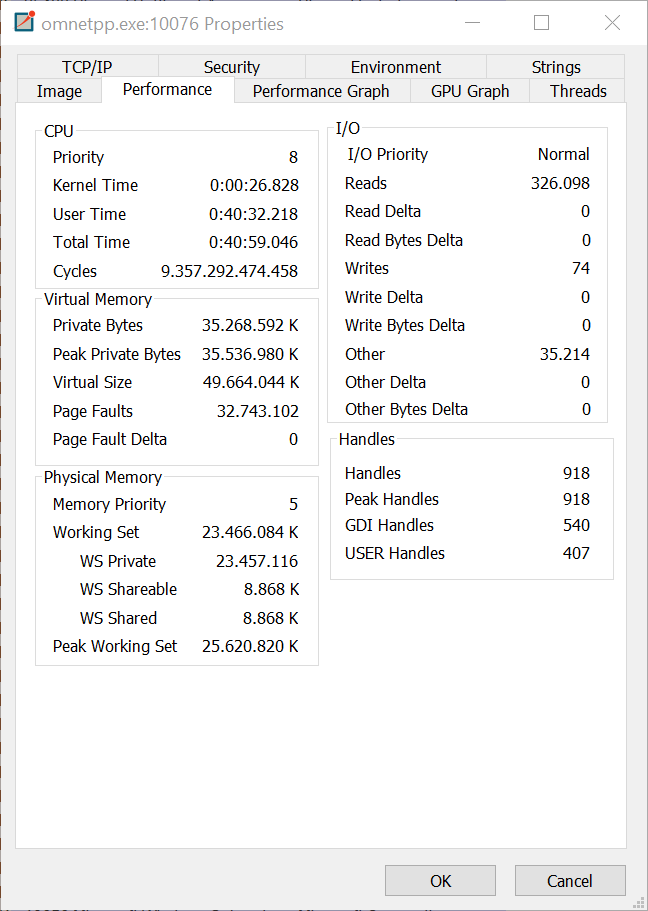
\includegraphics[width=\textwidth,height=0.7\textheight,keepaspectratio]{pic/OmnetPerformance}
	\end{center}
	
	\chapter{\glsentryname{omnetpp}-Zufallsverteilung}\label{app:zufallsverteilung}
	\section{Konfiguration}
	\begin{lstlisting}[language=INI, caption={[Erweiterte Durchläufe]}]
[Config KeinAngriffNoAttack]
extends = KeinAngriff
description = "Simulation ohne Angriff"

[Config KeinAngriffEmptyAttack]
extends = KeinAngriff
description = "Simulation ohne Angriff"
**.attackConfigurationFile = "attacks/empty.xml"

[Config KeinAngriffLateAttack]
extends = KeinAngriff
description = "Simulation ohne Angriff"
**.attackConfigurationFile = "attacks/late.xml"
	\end{lstlisting}
	\section{Ergebnis}
	\begin{center}
		\includesvg[width=\linewidth, keepaspectratio,inkscapelatex=false]{pic/VergleichVerschiedeneAngriffe} 
	\end{center}
	\chapter{\glsentryname{asl}-Message-Typen} \label{app:aslMessageTypen}
	Die hier gelisteten Messagetypen wurde aus einem Enum im Quellcode entnommen. Es müssen nicht zwingend alle Typen vollständig implementiert sein.
	\section{\glsentryname{layer5}}
	\begin{tiny}
		\begin{tabular}{|c|c|c|}
			\hline
			\rowcolor{Gainsboro!60}
			App.Type &         C++ Packet Object          & C++ controlInfo Object \\ \hline
			APP.0000 & cPacket("CreatedPacket-Layer5", 0) & UDPSendCommand()       \\ \hline
			APP.0001 & cPacket("CreatedPacket-Layer5", 0) & UDPBindCommand()       \\ \hline
			APP.0002 & cPacket("CreatedPacket-Layer5", 0) & UDPConnectCommand()    \\ \hline
			APP.0003 & cPacket("CreatedPacket-Layer5", 0) & UDPCloseCommand()      \\ \hline
			APP.0004 & cPacket("CreatedPacket-Layer5", 0) & UDPDataIndication()    \\ \hline
			APP.0005 & cPacket("CreatedPacket-Layer5", 0) & UDPErrorIndication()   \\ \hline
			APP.0100 & cPacket("CreatedPacket-Layer5", 0) & TCPSendCommand()       \\ \hline
			APP.0101 & cPacket("CreatedPacket-Layer5", 0) & TCPOpenCommand()       \\ \hline
			APP.0102 & cPacket("CreatedPacket-Layer5", 0) & TCPConnectInfo()       \\ \hline
			APP.0103 & cPacket("CreatedPacket-Layer5", 0) & TCPErrorInfo()         \\ \hline
			APP.0104 & cPacket("CreatedPacket-Layer5", 0) & TCPCommand()           \\ \hline
			APP.0200 &        TrafficLightStatus()\footnotemark[1]      & UDPSendCommand()       \\ \hline
			APP.0201 &        TrafficLightStatus()\footnotemark[1]     & UDPDataIndication()    \\ \hline
			APP.0300 &         TrafficLightCmd()\footnotemark[1]        & DPDataIndication()     \\ \hline
			APP.0301 &         TrafficLightCmd()\footnotemark[1]        & UDPSendCommand()       \\ \hline
			APP.1000 &        ApplicationPacket()         & UDPDataIndication()    \\ \hline
			APP.1001 &      SendApplicationPacket()       & UDPSendCommand()       \\ \hline
		\end{tabular}
	\end{tiny}
	\footnotetext[1]{Zugehörig zu dem Traffic-Light-Beispiel, mit dem \gls{seapp} vorgestellt wurde.}
	\section{\glsentryname{layer4}}
	\begin{tiny}
		\begin{tabular}{|c|c|c|}
			\hline
			\rowcolor{Gainsboro!60}
			TRA.Type &          C++ Packet Object          & C++ controlInfo Object \\ \hline
			TRA.0000 &  UDPPacket("CreatedPacket-UDP", 0)  &   IPv4ControlInfo()    \\ \hline
			TRA.0010 & TCPSegment("CreatedSegment-TCP", 0) &   IPv4ControlInfo()    \\ \hline
		\end{tabular}
	\end{tiny}
	\section{\glsentryname{layer3}}
	\begin{tiny}
		\begin{tabular}{|c|c|c|}
			\hline
			\rowcolor{Gainsboro!60}
			NET.Type &               C++  PacketObject                & C++ controlInfo Object \\ \hline
			NET.0000 & IPv4Datagram("Created packet-IPv4Datagram", 0) &     IPv4Datagram()     \\ \hline
			NET.0001 & IPv4Datagram("Created packet-IPv4Datagram", 0) &     Ieee802Ctrl()      \\ \hline
		\end{tabular}
	\end{tiny}
	\section{\glsentryname{layer2}}
	\begin{tiny}
		\begin{tabular}{|c|c|c|}
			\hline
			\rowcolor{Gainsboro!60}
			MAC.Type &                  C++ Packet Object                  & C++ controlInfo Object \\ \hline
			MAC.0000 &          PPPFrame("CreatedPacket-PPP", 0)           & null                   \\ \hline
			MAC.0010 & EthernetIIFrame("CreatedPacket-EthernetIIFrame", 0) & null                   \\ \hline
			MAC.0020 &   IdealAirFrame("CreatedPacket-IdealAirFrame", 0)   & null                   \\ \hline
			MAC.0030 &        AirFrame("CreatedPacket-AirFrame", 0)        & null                   \\ \hline
		\end{tabular}
	\end{tiny}
	
	\chapter{Auswertungen}\label{app:ende}
	\section{ARP}
	\subsection{Summe der Bits im studentischen Bereich}\label{app:arpStudenten}
	\begin{center}
		\includesvg[width=\linewidth, keepaspectratio,inkscapelatex=false]{pic/arp/ARPAngriffStudenten} 
	\end{center}
	\subsection{Angefangene ARP-Auslösungen}\label{app:initArp}
	\begin{center}
			\includesvg[width=\linewidth, keepaspectratio,inkscapelatex=false]{pic/arp/InitArpServer} 
	\end{center}
	\section{DoS}\label{app:dosTotalBits}
	\begin{center}
			\includesvg[width=\linewidth,  keepaspectratio,inkscapelatex=false]{pic/dos/TotalBitsAlle}
	\end{center}
\end{appendices}
